The references for this chapter include \cite{hurlbert2009}, \cite{dantzig1997}, \cite{dantzig2002}, \cite{chvatal1983}, as well as \cite{karmarkar1984}.

Usual introductions to the simplex algorithm start the following way : consider a company that has $ n $ products to sell. It shall produce nonnegative (not necessarily integral) amounts $ x_1,...,x_n $ of each product. To do so, the company makes use of $ m $ machines, each can respectively run $ b_1, ..., b_m $ minutes per month. Each product must pass though each machine, during an amount proportional to the quantity that must be produced : for each $ 1 \le j \le n $ and each $ 1 \le i \le m $, producing an amount $ x_j $ of the $ j $-th product requires machine $ i $ to run $ a_{ij}x_j $ minutes. So, the amounts $ x_j $ must satisfy the contraints
\[
    \forall i \in \{ 1,...,m \}, \sum_{j=1}^n a_{ij} x_j \leqslant b_i.
\]
Recall that the produced amounts can only be nonnegative, so we must also have
\[
    \forall j \in \{ 1,...,n \}, x_j \geqslant 0.
\]
Finally, the $ j $-th product will be sold at cost $ c_j $. The company then wants to maximize its profit
\[
    \sum_{j=1}^n c_j x_j.
\]
The motivates the Simplex problem.

\begin{problem}[Linear optimization problem]
    \textbf{Given} real numbers $ (a_{ij})_{\substack{1 \leq i \leq m \\ 1 \leq j \leq n}} $, $ (b_j)_{1 \leq j \leq n} $, $ (c_i)_{1 \leq i \leq m} $,

    \textbf{Maximize} over the real numbers $ x_1, ..., x_n $, the quantity
    \[
        \sum_{i=1}^n c_i x_i,
    \]

    \textbf{Under the constraints}
    \[
        \forall i \in \{ 1, ..., m \}, \sum_{j=1}^n a_{ij} x_j \leqslant b_i,
    \]
    \[
        \forall j \in \{ 1, ..., m \}, x_j \geqslant 0.
    \]
\end{problem}

This problem can be reformulated in its (obviously equivalent) matrix form

\begin{problem}[Linear optimization problem]
    \textbf{Given} a matrix $ A \in \mathbf R^{m \times n} $ and vectors $ b \in \mathbf R^m $, $ c \in \mathbf R^n $,

    \textbf{Maximize} over the vector $ x \in \mathbf R^n $, the linear form
    \[
        c^\top x,
    \]

    \textbf{Under the constraints}
    \[
        Ax \leqslant b,
    \]
    \[
        x \geqslant 0.
    \]
\end{problem}

Here, we have used the notation $ x \leqslant y $ to denote the condition $ x_i \leqslant y_i $ for all $ i \in \{ 1, ..., d \} $.

\begin{example}
    For instance, assume we want to maximize the linear form
    \[
        z = 400x + 200y
    \]
    under the constraints
    \[
        \left\{
        \begin{array}{ccc}
            30x + 20y \leqslant 6000 \\
            40x + 10y \leqslant 4000 
            x,y \geqslant 0
        \end{array}
        \right.
    \]
    Then, the problem can be represented as in the following drawing :

    \begin{center}
        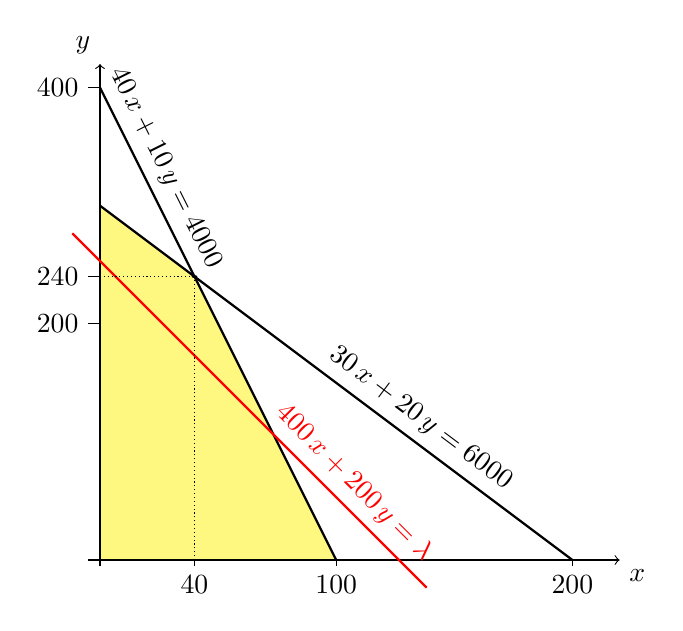
\begin{tikzpicture}[x=0.03cm,y=0.015cm]
            \fill[yellow!50] (0,0) -- (100,0) -- (40,240) -- (0,300) -- cycle;

            % Axes
            \draw[->] (-5,0) -- (220,0) node[below right] {$x$};
            \draw[->] (0,-5) -- (0,420) node[above left] {$y$};

            \foreach \x/\lab in {40/40,100/100,200/200}{
            \draw (\x,0) -- (\x,-5) node[below] {\lab};
            }

            \foreach \y/\lab in {200/200,240/240,400/400}{
            \draw (0,\y) -- (-5,\y) node[left] {\lab};
            }

            \draw[thick] (0,400) -- (100,0)
            node[pos=0.42,above left,sloped] {$40\,x + 10\,y = 4000$};

            \draw[thick] (0,300) -- (200,0)
            node[pos=0.65,above,sloped] {$30\,x + 20\,y = 6000$};

            \draw[thick,red,yshift=-10,xshift=-10] (0,300) -- (150,0)
            node[pos=0.75,above,sloped] {$400\,x + 200\,y = \lambda$};

            \fill (40,240) circle [radius=1.2];
            \draw[densely dotted] (40,0) -- (40,240);
            \draw[densely dotted] (0,240) -- (40,240);
        \end{tikzpicture}
    \end{center}

    The family of lines
    \[
        D_\lambda = \{ (x,y) \in \mathbf R^2, 400x + 200y = \lambda \}
    \]
    is a family of parallel lines. The problem is to find the maximum value of $ \lambda $ such that $ D_\lambda $ meets the regions of constraints.
\end{example}

Looking at the figure, it appears clear that the maximum is attained at the point of coordinates $ (40,240) $ which has been highlighted for that reason. The development of the Simplex algorithm establishes the following fact which applies to all situations.

\begin{theorem}
    If a linear optimization problem admits a solution, its optimal solution(s) exists and is(are) attained on a an extremal point of the constraints region.
\end{theorem}

On a side note, recall that :

\begin{proposition}\label{prop:extremal-points}
    Let $ C $ be a convex region of a real vector space. Let $ x \in C $. Then, the following assertions are equivalent :

    (i) For all $ a,b \in C $, if $ x = \frac 1 2 (a+b) $, then $ x = a $ or $ x = b $,

    (ii) For all $ a,b \in C $, if $ x \in [a,b] $, then $ x = a $ or $ x = b $,

    (iii) $ C - \{ x \} $ is convex.
\end{proposition}

\begin{proof}
    $ (i) \implies (ii) $
    
    Let $ a,b \in C $ and assume $ x \in [a,b] $. We have $ x = \lambda a + (1-\lambda) b $ for some $ \lambda \in [0,1] $.

    Assume that $ \lambda \neq \frac 1 2 $. Without loss of generality, we can assume $ \lambda < \frac 1 2 $. Then, $ 2\lambda \in [0,1] $, so $ 2\lambda a + (1-2\lambda) b \in [a,b] $.

    But, we have
    \[
        \frac 1 2 (b + 2\lambda a + (1-2\lambda)b) = \frac 1 2 (2b + 2\lambda a - 2\lambda b) = b + \lambda (a - b) = x
    \]
    So, $ x $ is the middlepoint of $ b $ and $ \frac 1 2 (b + 2\lambda a + (1-2\lambda)b) $. As a result, we have either $ x = b $ or $ b = \frac 1 2 (b + 2\lambda a + (1-2\lambda)b )$.

    Simplifying $ b = \frac 1 2 (b + 2\lambda a + (1-2\lambda)b ) $ yields $ b = b + \lambda (a - b) = x $, so in both cases, $ x = b $ and we have the result.

    $ (ii) \implies (iii) $
    
    Let $ a,b \in C - \{ x \} $. Let $ \lambda \in [0,1] $. Then, we cannot have $ \lambda a + (1-\lambda) b = x $, because this would imply either $ x = a $ or $ x = b $, which are both false by assumption. Moreover, since $ C $ is convex, $ \lambda a + (1-\lambda) b \in C $. So finally, $ \lambda a + (1-\lambda) b \in C - \{ x \}$. 
    
    $ (iii) \implies (i) $

    Let $ a,b \in C $, assume that $ x = \frac 1 2 (a+b) $. Assume that $ x \neq a $ and $ x \neq b $. Since $ C - \{ x \} $ is convex, we have $ \frac{a+b}{2} = x \in C - \{ x \}$, a contradiction.
\end{proof}

\begin{definition}[Extremal point of a convex region]
    Given a convex region $ C $ of say $ \mathbf R^d $, $ x \in C $ is said to be an \textit{extremal point} of $ C $ if one of the equivalent propositions of Proposition~\ref{prop:extremal-points} is satisfied.
\end{definition}

\begin{remark}
    Note that the constraints are nonstrict inequalities. Allowing strict inequalities would yield the constraints polyhedron to be non-closed, hence non-compact, and as such, there could be no solution. At any rate, we believe that it is of no use to optimize on non-closed domains---in most cases, taking the doesn't change much and yields the same result with the benefit of having the theoretical guarantee that an optimizer exists (if the region is bounded, i.e., compact).
\end{remark}

\begin{remark}
    Linear optimization finds its interest in optimizing linear functions over linear constraints. This essentially means that the function that has to be optimized is linear, and since optimizing vectors does not really make sense so far, the function essentially ought to be a linear form. Furthermore, the constraint must be linear, in the sense that they must be written $ g_i(x) \leqslant b_i $, where $ g_i $ are linear, and real-valued---hence, linear forms.

    Note that writing down a linear optimization problem will not necessarily result in the form that has been given above.

    The above form of linear optimization problems is called \textit{standard form}. When we are dealing an optimization problem the objective function and constraint functions of which are all linear, it will often not be in standard form in the beginning. It is important to reformulate them and rewrite them this way, in order for Dantzig's Simplex algorithm to work. This is done by applying, for instance, a couple of the following changes:

    \begin{itemize}
        \item If the problem asks for minimization instead of maximization, maximize the opposite of the objective function.
        
        \item If the inequalities are not in the right direction, multiply by $ -1 $. 

        \item Equality constraints $ \sum_{j=1}^n a_{ij}x_j = b_i $ ($ Ax = b $) are just two in equality constraints $ \sum_{j=1}^n a_{ij}x_j \leqslant b_i $ ($ Ax \leqslant b $) and $ \sum_{j=1}^n (-a_{ij})x_j \leqslant -b_i $ ($ -Ax \leqslant -b $)

        \item Replace constraints of the form $ x \geqslant \alpha $ by $ y := x - \alpha \geqslant 0$ to match the positivity constraint of the standard form.

        \item Replace constraints of the form $ x \leqslant \beta $ by $ y := x - \beta \leqslant 0$ to match the positivity constraint of the standard form.

        \item Exchange twice-constrained variables $ \alpha \leqslant x \beta $ by $ y := x - \alpha \geqslant $, adding the constraint $ y \leqslant \beta - \alpha $ (which is equivalent to adding a row with $ 0 $'s and a $ 1 $ at the right position in $ A $, as well as a $ \beta - \alpha $ on the same row in the vector $ b $). If there are several such constraints, their intersection is a constraint of the same form (intersections of real-line segments remain segments).

        \item Unconstrained variables $ x $ are a difference of two constrained variables $ x = x^+ - x^- $ with $ x^+, x^- \geqslant 0 $.
    \end{itemize}

    Using these tricks, all linear programming problems can be reduced to standard form. As a result, developing an algorithm that solves a linear programming problem in standard problem is sufficient to solve them all.
\end{remark}